\section{Graph-based Input Representation}
%\label{sec:RelatedWork}

\cite{StringExpr} --- regular expressions (analysis -> CFG -> regular approximation)
\cite{AbstrParsing} --- dataflow equations
\cite{ALVOR1,ALVOR2} --- regular expressions

Also we suppose that input data structure for parser is direct acyclic graph (DAG) with one source and 
one sink vertices. Our experience of dynamic SQL translation for real information system shows that DAG 
is a good approximation of the dynamically constructed expressions set for practical use. We should replace 
all cycles with single repetition during approximation to get such graph. This way we can process all vertices 
in the topological order and avoid the problem with cycles processing previously discussed.

In the general case input graph can be arbitrary graph with cycles~\cite{AbstrParsing}. Cycles in the input graph may 
be cause of infinite parsing. ut we have not found any practice implementations with problem of cycles processing fully 
solved. We have found only two known implementations of abstract parsing: Alvor\footnote{Alvor is an Eclipse IDE plug-in 
for statically checking of string-embedded SQL queries in Java programming language. This plug-in is based on LALR and GLR 
abstract parsing and can be used either for incremental analysis or for offline checking of full code base. Alvor project 
web site: \href{http://code.google.com/p/alvor/}{http://code.google.com/p/alvor/}} and the tool described in the Doh, Kim, 
and Schmid's article. Alvor use stack size limitation to avoid infinite processing of cycles. Doh, Kim, and Schmid's 
implementation of LALR(1)-based abstract parsing cannot be found and article does not contain practice solution of 
cycles processing problem. In sum, efficient arbitrary graph with cycles processing in abstract parsing is an open question.
	

%For practical usage it is very important that information systems can contain a big 
%number of dynamic queries and each one of them can contains hundreds of 
%branches~\cite{TiunovaUIInt}. The necessity of analyzing all possible values for 
%each query can cause  performance problems and exponential growth of required 
%resources.

In our approach 

We suppose that input data structure for abstract analysis is a graph which represents the result of constant
propagation: every path in input graph corresponds with one of possible values of dynamic query. Let we define 
that this path produce corresponded value and we will say that query contains lexical or syntax error if at least 
one path which produce value with error exists in the corresponding graph. After that we define that input graph 
tokenization or lexical analysis is the process which convert input graph with string labels on edges (picture~\ref{pic1}) 
to graph with tokens. The same way we define parsing or syntax analysis as the process which produce parsing forest by 
input graph with edges labeled with tokens. As a result of parsing we have forest where each tree corresponds with query 
value produced by any path in the input graph. When we describe abstract parsing and translation we assume that input 
graph tokenization performed successfully.


One of the most popular examples of string-embedded languages is a dynamic SQL, and we will use it for all 
examples in this article. Let we try to process the some code presented below which construct and execute 
dynamic SQL query.  

\begin{verbatim} 
(1) IF @X = @Y
(2) SET @TABLE = '#tbl1'
(3) ELSE
(4) SET @TABLE = 'tbl2'
(5) SET @S = 'SELECT x FROM ' + @TABLE
(6) EXECUTE (@S)
\end{verbatim}

Variable \verb @S \ contains dynamically generated query and has 2 possible values at the point of query execution. 
During approximation we can get a graph which presents the set of the possible values of the variable \verb @S \ at the 
line 6. Each edge of this graph contains string which represent a part of query. Note that real-world systems can communicate
 with other systems source of which may be inaccessible to analyze. These systems can contain parts of queries 
to process and we should use some approximations. For example, clients applications of information system can 
sent conditions for filters (conditions for \verb|where| clause of \verb|select| statement) as part of requests.  
Graph for our code is presented in picture~\ref{pic1}.

\begin{figure}
    \begin{center}
        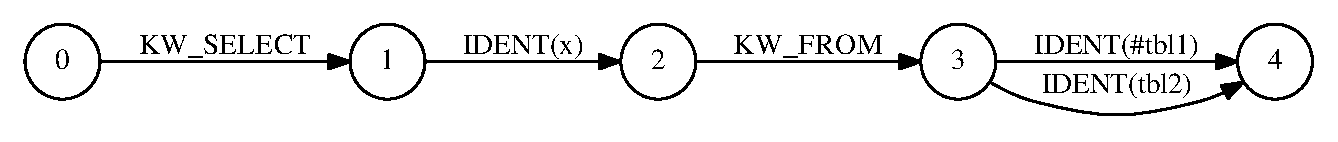
\includegraphics[width=11cm,height=1.1cm]{graphs/simple_sql.eps}
        \caption{Example of graph for dynamic query.}
        \label{pic1}        
    \end{center}
\end{figure}

Abstract parsing is based on the idea of reusing of the control structures utilized in the classical parsing with the 
implementation of special mechanism of their interpretation. Control tables for the analyzer (action, goto) may be generated by
 the language specification by using some standard tool i.e. Yacc~\footnote{Yacc is a classical LALR-based parsers generator. 
Yacc web site: \href{http://dinosaur.compilertools.net/}{http://dinosaur.compilertools.net/}}. LR automaton~\cite{Grune} should
 be modified so that it is able to compute all possible parser states for each vertex of the graph~\cite{AbstrParsing}. 
So, the basic idea of the abstract parsing is a graph processing with fix-point calculation~\cite{ALVOR2}.

Let we use the grammar presented below to generate syntax analyzer.

\begin{verbatim}
s -> Ae
e -> BD
e -> CD
\end{verbatim}

Input for generated analyzer is the graph presented in picture~\ref{pic2}. The set of parser states for each vertex for 
graph will be calculated during syntax analysis. Result of states calculation shown in the picture ~\ref{pic3}.

\begin{figure}
    \begin{center}
        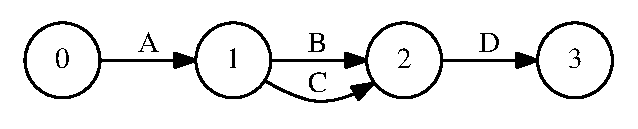
\includegraphics[width=7cm,height=1.5cm]{graphs/simple_grammar_inpt.eps}
        \caption{Input graph for abstract parsing.}
        \label{pic2}
    \end{center}
\end{figure}

\begin{figure}
    \begin{center}
        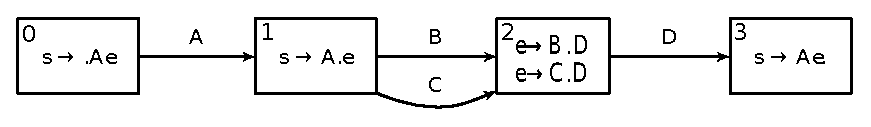
\includegraphics[width=11cm,height=1.5cm]{graphs/simple_grammar_items.eps}
        \caption{Parser states for input graph which presented in picture~\ref{pic2}.}
        \label{pic3}
    \end{center}
\end{figure}

So, there is an algorithm for syntax analysis of string-embedded languages. Note, that the problem of static 
analysis if dynamically generated strings could not be solved in the common case~\cite{ALVOR2}. Also there are 
possible two implementation of abstract parsing algorithm except our one. Note that these tools do not solve 
the problem of string-embedded statements translation.


